\chapter{Implementation and Results}
\label{chapter:implementation}

I implemented two example cases: a mobile web application for a
developer conference and a networking library for data caching and
fetching multiple times. Here I present the architecture, components
and the implementation details I used for fulfilling the requirements
listed in Chapter~\ref{chapter:methods} and the techniques I used and
the compromises I had to make to tackle the problems in mobile web
development. I used tools introduced in
Chapter~\ref{chapter:tools-and-techniques} and APIs introduced in
Chapter~\ref{chapter:html5} and
Chapter~\ref{chapter:other-related-specifications}.

\section{Conference Application}

\begin{figure}[h!]
  \begin{center}
    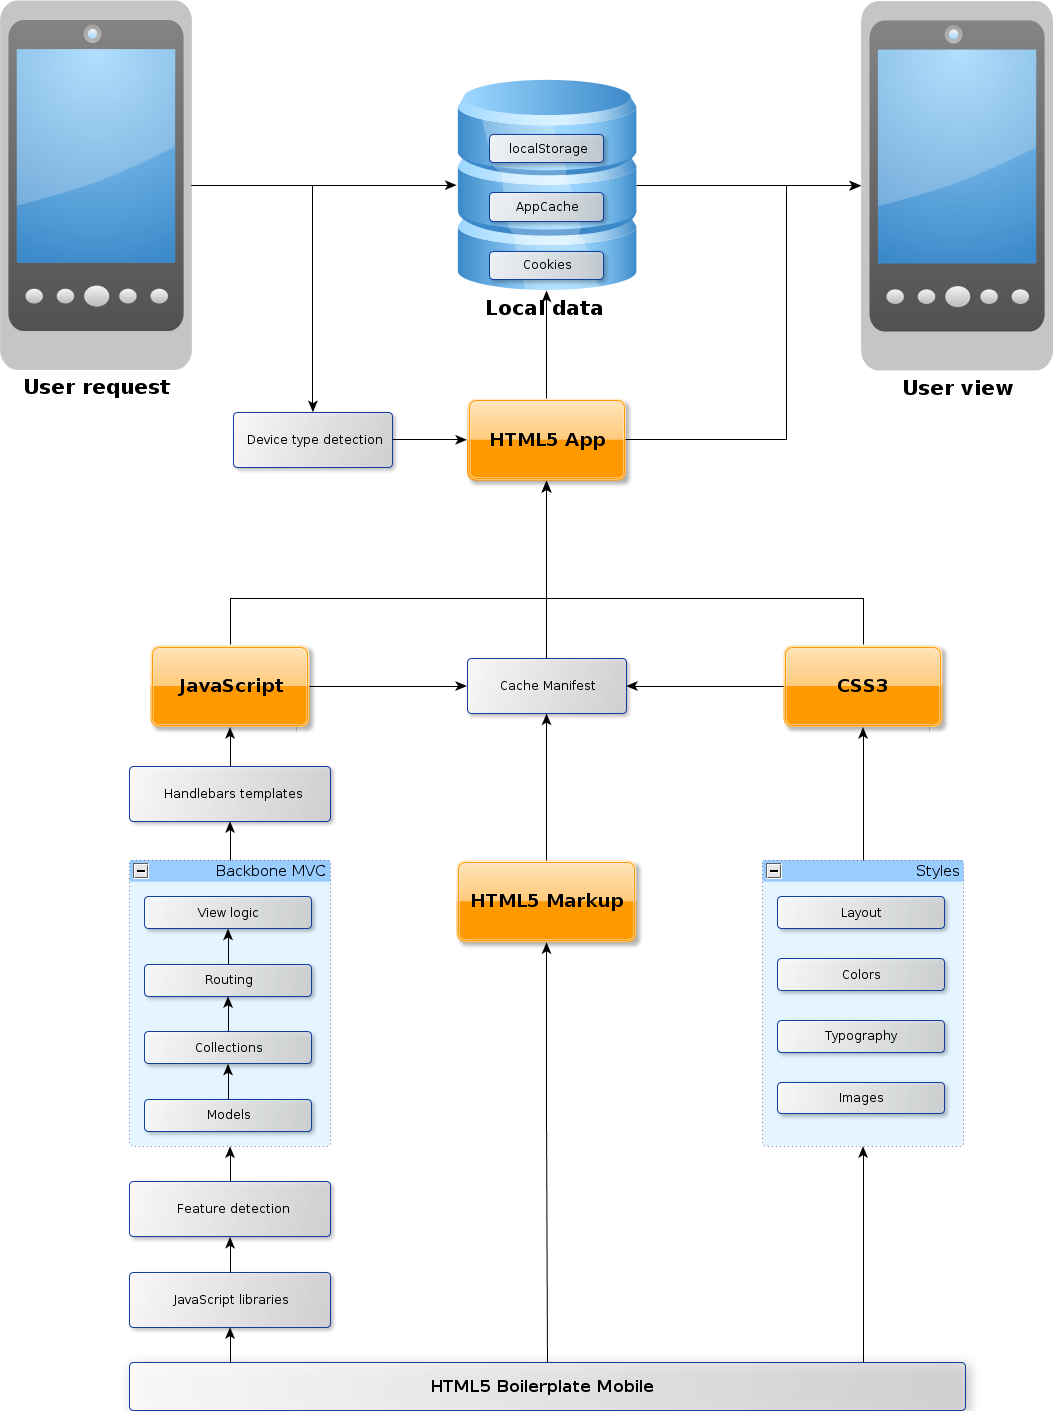
\includegraphics[width=\textwidth]{images/devdays.png}
    \caption{Conference schedule application architecture.}
    \label{figure:devdays.png}
  \end{center}
\end{figure}

The conference
schedule\footnote{\url{http://m.qtdevdays2011.qt.nokia.com/}} is a
single-page application (see
Section~\ref{section:single-page-applications}) with a lightweight
backend written in Python using the Django Web
Framework\footnote{\url{https://www.djangoproject.com/}}.

The backend provides the static assets (JavaScript, \abbr{CSS},
images, etc.) and an \abbr{API} for persisting session feedback to a
MySQL\footnote{\url{http://www.mysql.com/}} relational database. It
also generates the HTML5 AppCache (see Section~\ref{section:appcache})
offline cache manifest file based on the categorized device type.

The frontend is a JavaScript application written using the
Backbone\footnote{\url{http://backbonejs.org/}} \abbr{MVC} framework
(see Section~\ref{section:js-mvc}). Other JavaScript libraries include
Underscore\footnote{\url{http://underscorejs.org/}} for data
manipulation, jQuery\footnote{\url{http://jquery.com/}} for \abbr{DOM}
API abstraction, Handlebars\footnote{\url{http://handlebarsjs.com/}}
for templating, and
Modernizr\footnote{\url{http://www.modernizr.com/}} for feature
detection. The HTML5 Mobile
Boilerplate\footnote{\url{http://html5boilerplate.com/mobile}} was
used as an initial markup structure for the application. The
architecture of the application is shown in
Figure~\ref{figure:devdays.png}. Wireless networks can be unreliable
in conference settings, so offline support was also added using
several different JavaScript techniques and HTML5 APIs.

The application was designed for touch screens on various platforms
and screen sizes. The layout adjusts to the available space and
provides rich interactive components. Integration to social networking
services was also added as an additional
functionality. Figure~\ref{figure:ipad-session.jpg} shows an example
view in the application.

\begin{figure}[h!]
  \begin{center}
    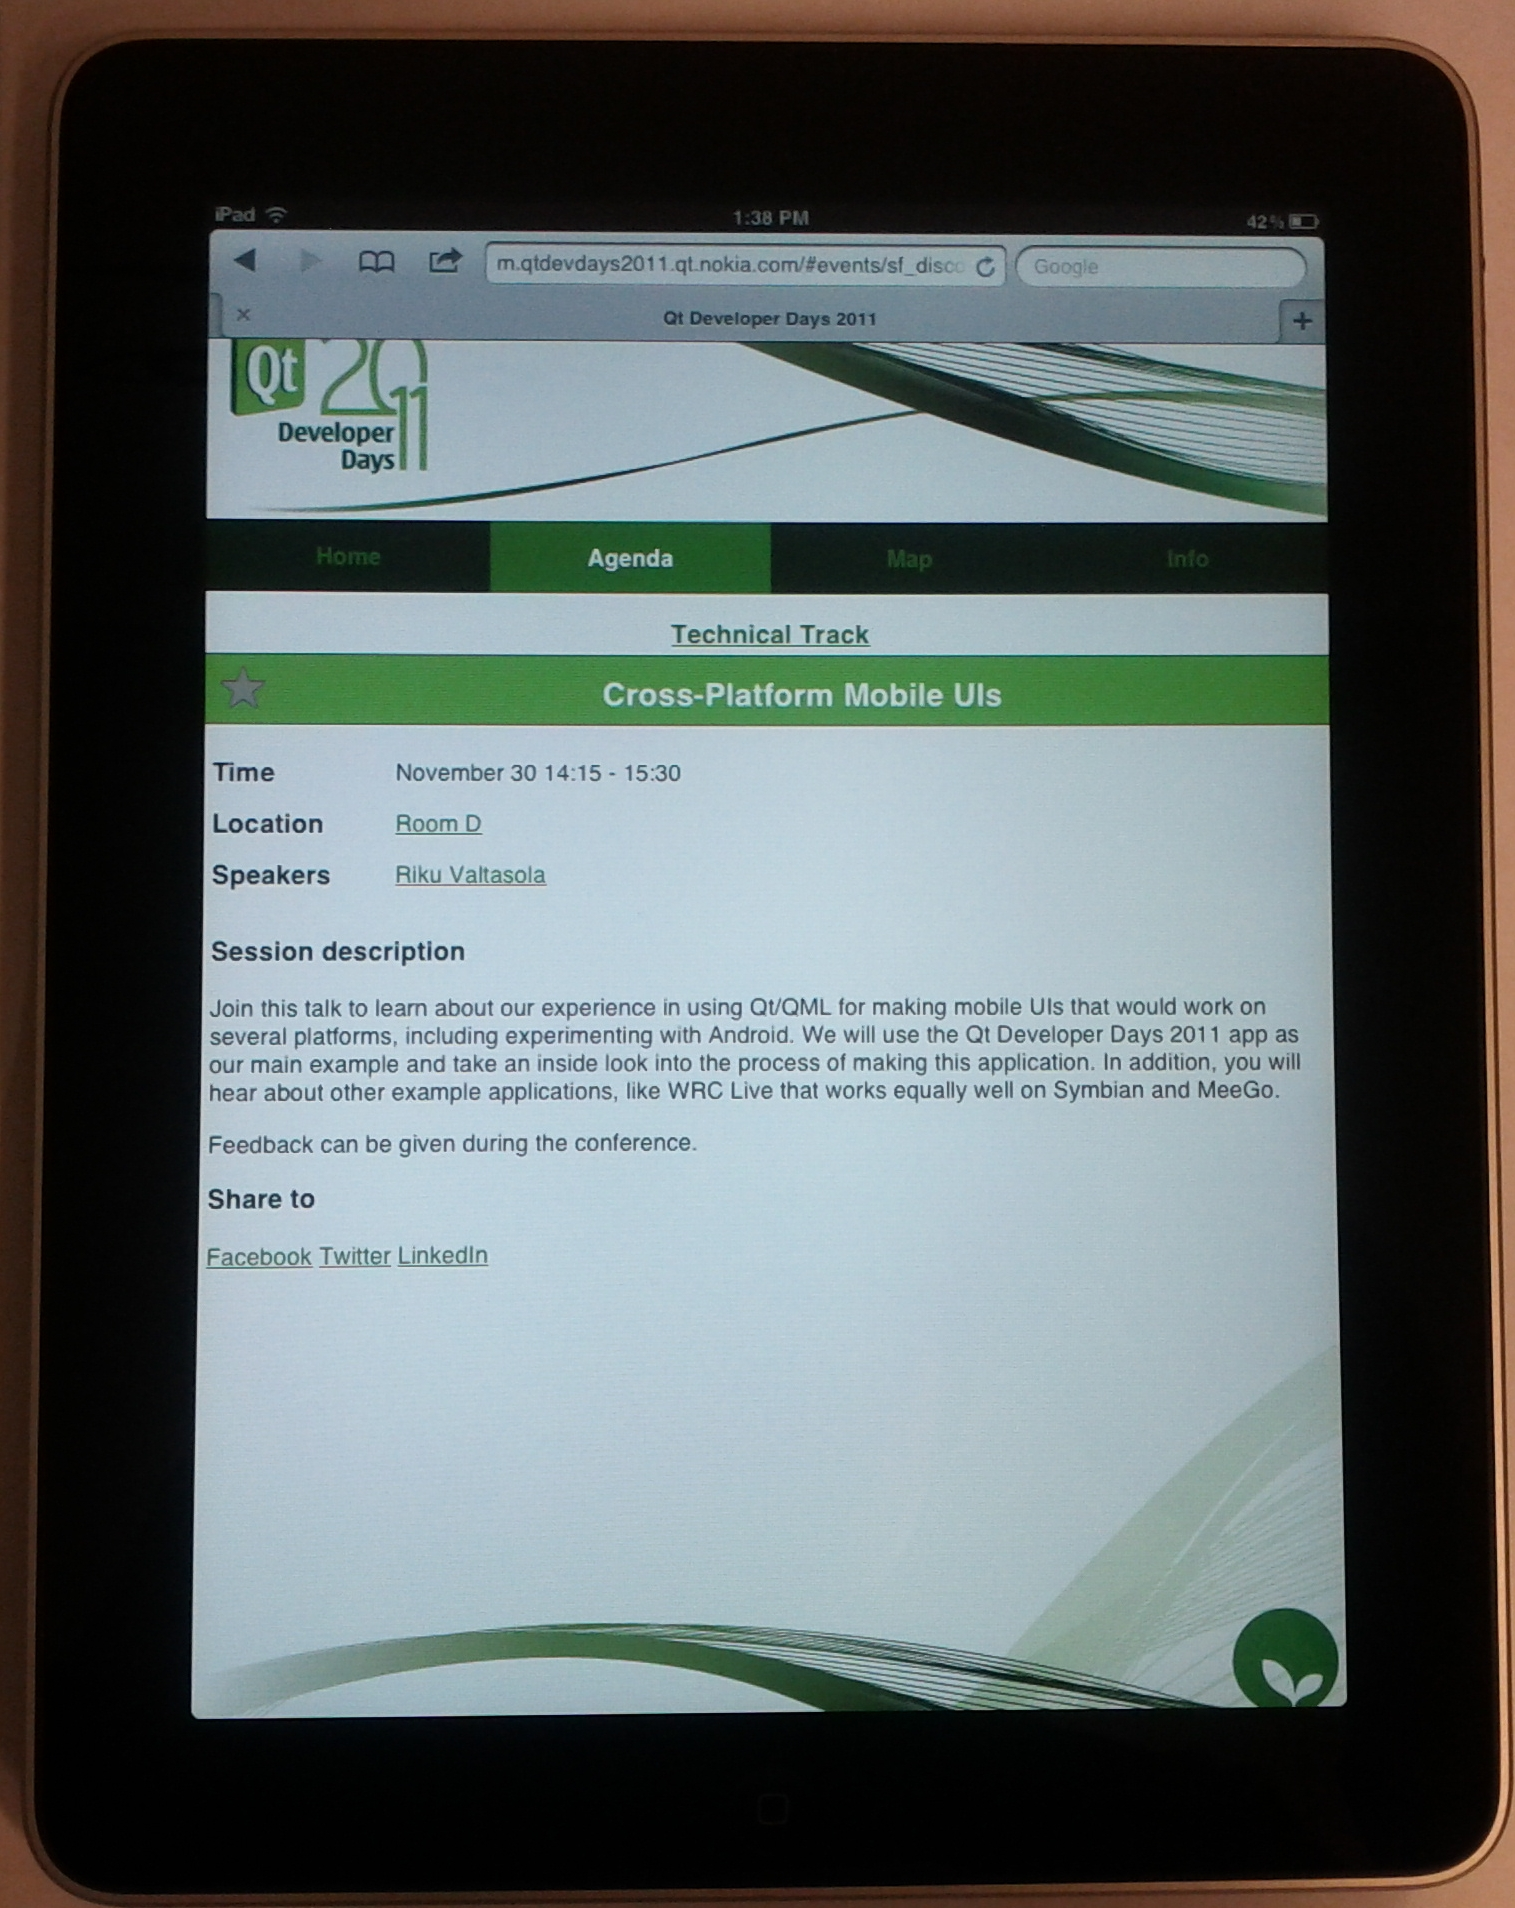
\includegraphics[width=\textwidth]{images/ipad-session.jpg}
    \caption{Session details view on an iPad.}
    \label{figure:ipad-session.jpg}
  \end{center}
\end{figure}

\section{JSONCache JavaScript Library}
\label{section:jsoncache}

JSONCache is a lightweight JavaScript library for fetching \abbr{JSON}
data in unreliable networks. The library was designed especially to
handle unreliable mobile networks with connection problems and short
interruptions. The goal is to avoid networking as long as possible and
failing gracefully if the network connection is not stable.

JSONCache provides two main functionalities: data caching and
attempting to fetch the data multiple times.

The caching layer uses the client side localStorage (see
Section~\ref{section:datastorage}) cache of \abbr{HTML5}. Data
requests can be done using the JSONCache \abbr{API} which always
checks the local cache first before opening any network
connections. If the data is already in the cache, the cached data is
checked for validity and if the data is not expired, it is returned
immediately. If the data is not in the cache or it is expired, a new
network request is made and the received data is cached and
returned. The expiration time of a data item can be configured in the
library settings.

JSONCache also tries to fetch the data multiple times to handle small
interruptions in network connections.  For example, when a user leaves
his or her work place and uses a web application, the mobile device
changes from the workplace \abbr{WiFi} network to the \abbr{3G}
network, there is a short interruption in the connection, and any
ongoing network requests are affected.

If a data fetch fails, a new fetch is issued after a timeout (defined
in the configuration). On subsequent attempts the timeout is
increased, and after a defined number of attempts the fetch error is
issued.

Figure~\ref{figure:jsoncache-demo.png} shows an interactive demo of
the JSONCache library. The
demo\footnote{\url{http://kpuputti.github.com/JSONCache/demo/index.html}}
simulates the caching and fetching functionality of the library by
demonstrating an unreliable network based on the configuration.

\begin{figure}[h!]
  \begin{center}
    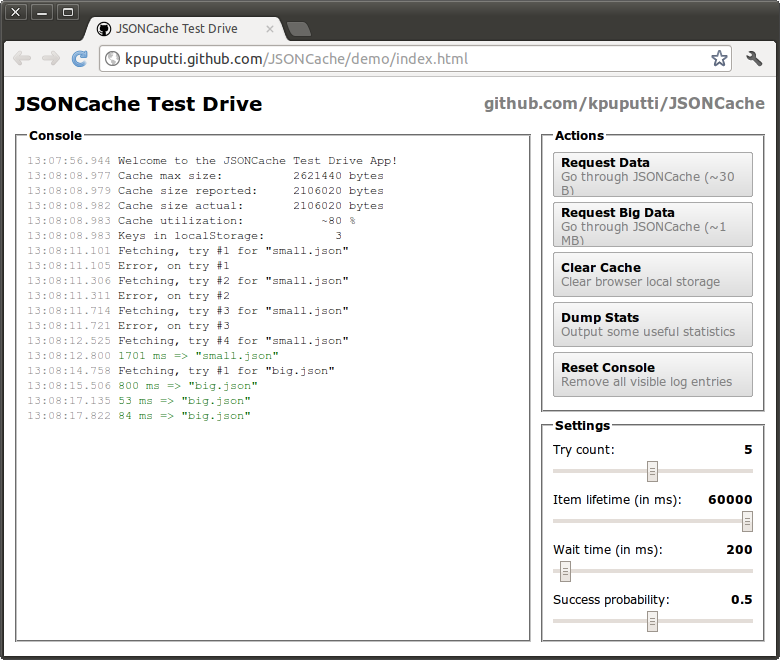
\includegraphics[width=\textwidth]{images/jsoncache-demo.png}
    \caption{Interactive JSONCache demo.}
    \label{figure:jsoncache-demo.png}
  \end{center}
\end{figure}

\section{Targeting Different Platforms}
\label{section:targeting-platforms}

Despite the web browser being the unified environment for different
platforms, there are lots of differences between various devices. The
form factors vary from tiny mobile screens to touch screen tablets and
desktop monitors and each device and platform has its own feature
set. Browsers also have known bugs that have to be handled.

Therefore, means to detect the user's device are needed (see
requirements 1 and 2 in
Section~\ref{section:devdays-requirements}). Here I present two such
means: device detection and feature detection. Both of these were used
in our conference application.

\subsection{Device Detection}
\label{subsection:device-detection}

The User-Agent (\abbr{UA}) \abbr{HTTP} header contains detailed
information of the web browser and the platform where the request
originates from. As can be seen from Table~6.1\tableref, we can
extract platform- and browser-specific information from the UA header.

\begin{table}
  \begin{tabular}{ l | l | p{7cm} }
    \textbf{Device} & \textbf{Platform} & \textbf{User-Agent} \\ \hline
    Samsung Nexus S & Android 2.3.4 & Mozilla/5.0 (Linux; U; Android 2.3.4; en-us; Nexus S Build/GRJ22) AppleWebKit/533.1 (KHTML, like Gecko) Version/4.0 Mobile Safari/533.1 \\ \hline
    Apple iPhone & iOS 3.1.3 & Mozilla/5.0 (iPhone; U; CPU iPhone OS 3\_1\_3 like Mac OS X; de-de) AppleWebKit/528.18 (KHTML, like Gecko) Version/4.0 Mobile/7E18 Safari/528.16 \\ \hline
    Apple iPad & iOS 5.0 & Mozilla/5.0 (iPad; CPU OS 5\_0 like Mac OS X) AppleWebKit/534.46 (KHTML, like Gecko) Mobile/9A334 \\ \hline
    Unknown & Android & Opera/9.80 (Android; Opera Mini/6.5.26571/26.1023; U; de) Presto/2.8.119 Version/10.54 \\ \hline
  \end{tabular}
  \label{table:user-agents}
  \caption{Example User-Agent strings.}
\end{table}

In the conference application, device detection was used in the
backend to provide a different offline AppCache manifest (see
Section~\ref{section:appcache}) to different device groups. The
detection was also used in defining the assets to be preloaded in the
application. The devices were divided into four categories based on
the rules defined in Table~6.2\tableref. There were serious
limitations in this approach, and compromises had to be made.

First, there is no way to surely know if the device actually is what
it reports itself to be. Second, the most important thing to know when
generating the screen-specific assets in the manifest file would have
been the screen size. However, this information is not present in the
UA header. I could have listed all the assets for all the devices, but
then the list of offline assets would have grown too much and, for
example, have large images also for older mobile phones.

Despite the drawbacks, the received advantages of this approach
outweighed the possible compromises. The worst that could happen was
that the device was wrongly classified and some graphics assets were
not downloaded for offline use.

\begin{table}
  \begin{tabular}{ l | l }
    \textbf{Rule} & \textbf{Device Type} \\ \hline
    'iPad' in UA & highres \\
    'iPhone' in UA & iphone \\
    'Android 3' in UA & highres \\
    'mobile' (case insensitive) in UA & mobile \\
    'MIDP' in UA & mobile \\
    'Opera Mobi' in UA & mobile \\
    'Opera Mini' in UA & mobile \\
    otherwise (desktop computer) & highres
  \end{tabular}
  \label{table:device-detection-rules}
  \caption{Device type detection rules.}
\end{table}

Getting platform and browser information from the UA header might look
tempting and useful, but it is considered a bad practice to detect a
device from it and providing device-specific bug fixes or additional
features. The header can easily be changed and some browsers or
browser plugins even provide preconfigured values for certain browsers
or devices for spoofing. Also, the device-specific bug fixes might
become obsolete with browser and platform updates, and the application
might break due to invalid expectations. This is why feature detection
is generally the recommended option whenever possible.

\subsection{Feature Detection}
\label{section:feature-detection}

Feature detection is an important concept in designing with
progressive enhancement (See
Section~\ref{subsection:progressive-enhancement}). A lot of the
HTML5-related JavaScript APIs are still unsupported in several
platforms, but browser developers are constantly filling in the
gaps. Therefore, it is important to check whether a certain feature is
supported and to provide graceful fallback mechanisms for browsers
lacking the functionality.

Doing run-time feature detection provides the possibility to give
additional functionality to modern browsers and instant support for
devices that add the support for the feature in the lifetime of the
application. In the conference application, I used the Modernizr
feature detection library\footnote{\url{http://www.modernizr.com/}} to
check for HTML5 features.

For example, the user could add sessions to his or her favorites by
clicking the star in the agenda (see
Figure~\ref{figure:iphone-android-agenda.jpg}) or on the session
details view. The favorites were then listed on the home view (see
Figure~\ref{figure:android-home-favorites.jpg}) together with
information about the time left for them to begin (see requirements 3
and 6 in Section~\ref{section:devdays-requirements}).

\begin{figure}[h!]
  \begin{center}
    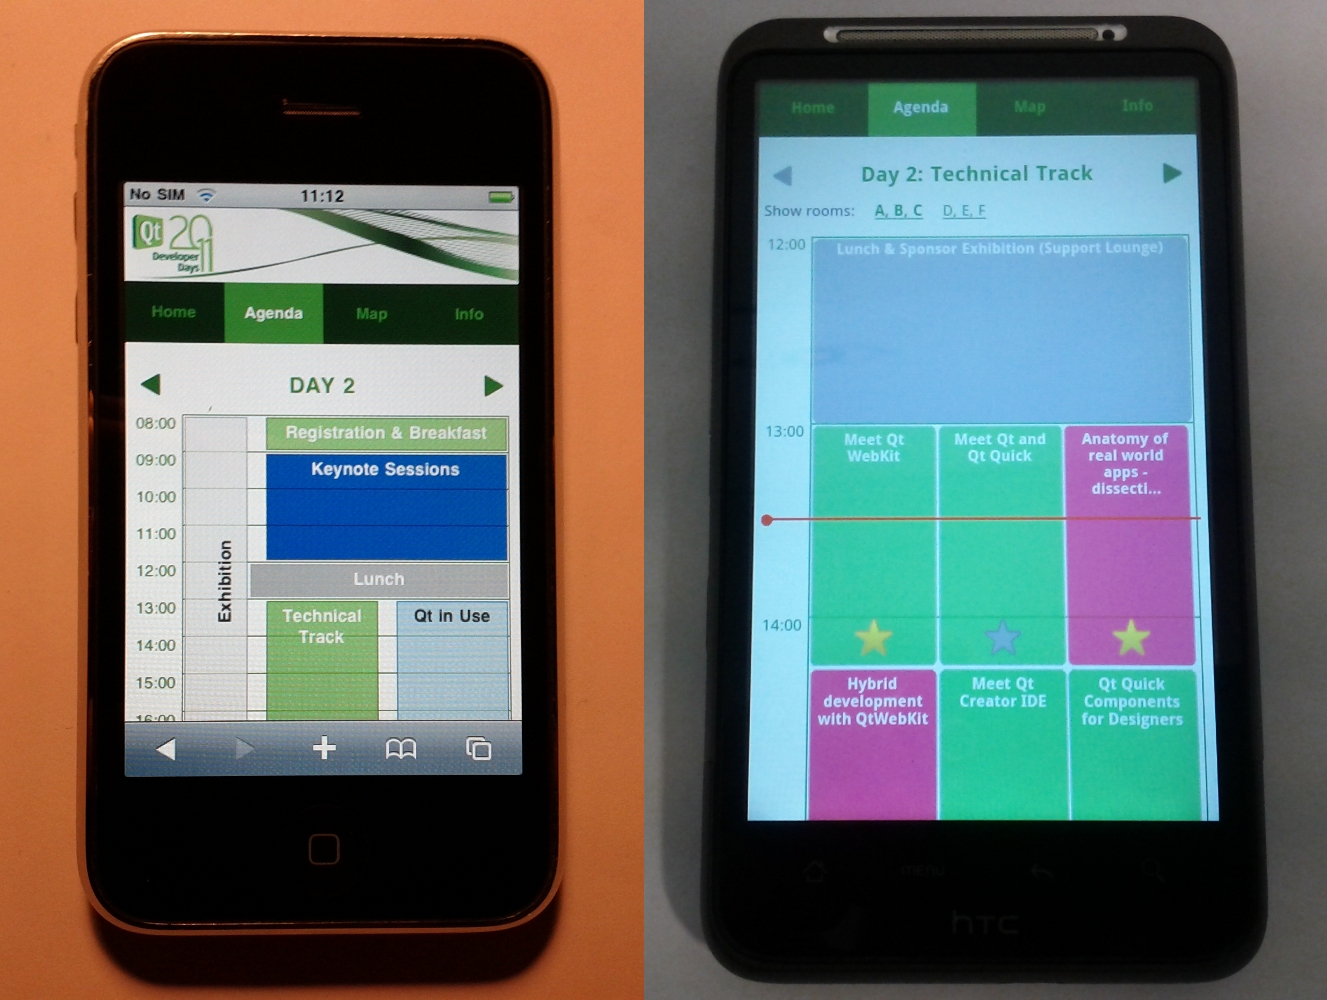
\includegraphics[width=\textwidth]{images/iphone-android-agenda.jpg}
    \caption{Agenda view with stars to add favorites on an iPhone
      (left) and on a device running Android (right).}
    \label{figure:iphone-android-agenda.jpg}
  \end{center}
\end{figure}

\begin{figure}[h!]
  \begin{center}
    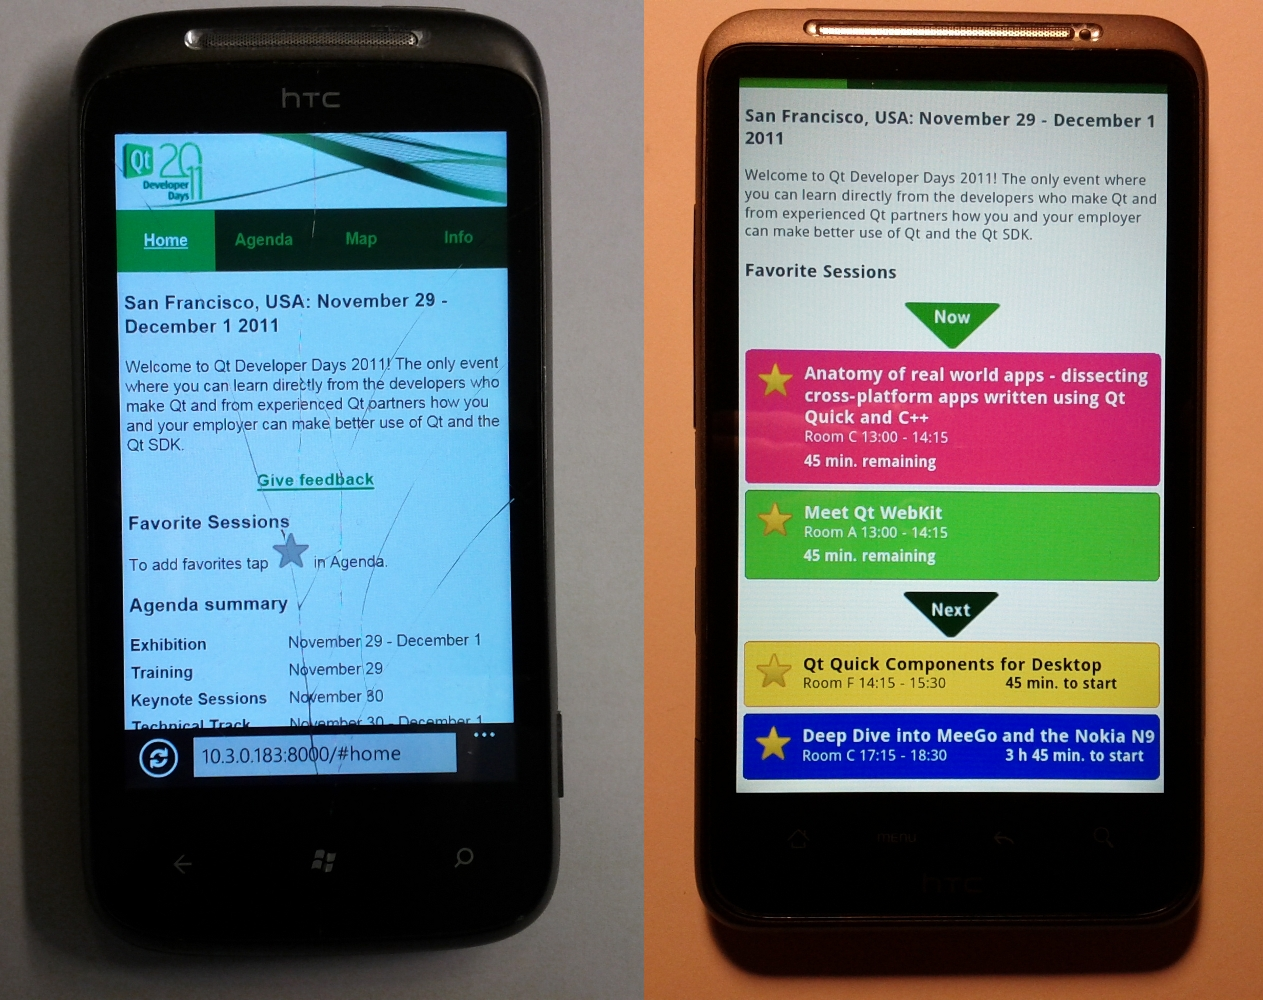
\includegraphics[width=\textwidth]{images/android-home.jpg}
    \caption{Home view without favorites (left) on a device running
      Windows Phone 7 and with favorites (right) on a device running
      Android.}
    \label{figure:android-home-favorites.jpg}
  \end{center}
\end{figure}

I used HTML5 localStorage for storing the favorites in the user's web
browser. By using Modernizr, I detected localStorage support and
showed the favorite stars only in browsers that supported the
functionality. For all other browsers, the stars were simply hidden
and users could not add favorites.

\section{Targeting Different Screens}
\label{section:targeting-screens}

Probably the biggest difference in various devices and form factors is
the screen and its size, resolution, and dimensions. Web applications
should adjust to the available space and flexibly handle screen
orientation and window size changes (see requirement 2 in
Section~\ref{section:devdays-requirements}).

First, to target mobile and tablet platforms, the viewport meta
information should be indicated in the document. The following tag was
used in the conference application:

\begin{verbatim}
<meta name="viewport" content="width=device-width,
                               initial-scale=1.0">
\end{verbatim}

The viewport meta tag was first introduced in Apple's iPhone and
afterwards ported to other platforms, such as Android. The possible
configuration options and default values might vary between
platforms. Values accepted by Android are shown in
Table~6.3\tableref. iOS devices also support these same properties.

\begin{table}
  \begin{tabular}{ l | l | p{5cm} }
    \textbf{Property} & \textbf{Description} & \textbf{Value} \\ \hline
    height & Height of the viewport. & pixel value or 'device-height' \\
    width & Width of the viewport. & pixel value or 'device-width' \\
    initial-scale & Initial zoom level. & float value (0.01--10) \\
    minimum-scale & Minimum zoom level. & float value (0.01--10) \\
    maximum-scale & Maximum zoom level. & float value (0.01--10) \\
    user-scalable & Enables/disables zoom. & 'yes' or 'no' \\
    target-densitydpi & Visual pixel density. & dpi value, 'device-dpi', 'high-dpi', 'medium-dpi', or 'low-dpi' \\
  \end{tabular}
  \label{table:viewport-meta}
  \caption{Viewport meta tag configuration for Android according to
    \url{http://developer.android.com/guide/webapps/targeting.html}}
\end{table}

If I do not set the viewport configuration tag, the device uses its
own default values for the properties. For example, the default value
for the width property is 980 pixels in
iOS\footnote{\url{https://developer.apple.com/library/safari/documentation/appleapplications/reference/SafariHTMLRef/Articles/MetaTags.html}},
which is clearly defined for web sites targeting desktop
browsers. Without setting this value to something smaller and more
appropriate in a mobile context, the whole application is very wide
and has small and unreadable text in the initial zoom level.

In the viewport configuration I used for the conference application
(as defined above), I set the viewport width to 'device-width'. This
makes the application width to adjust to the visual pixels of the
device screen and works well with screens of different sizes and
dimensions. The only other viewport property I set is the initial
scaling. This is set to 1.0 to force the browser to render the
application without any initial zooming.

In addition to the viewport configuration, I used media queries (see
Section~\ref{section:css}) to use better background images for
high-resolution screens. I also dynamically set the map view (see
Figure~\ref{figure:nokia-map.jpg}) images based on the screen
dimensions so that I could provide smaller images for smaller screens
and high resolution images for tablets and other devices with larger
screen estate (see requirement 5 in
Section~\ref{section:devdays-requirements}).

\begin{figure}[h!]
  \begin{center}
    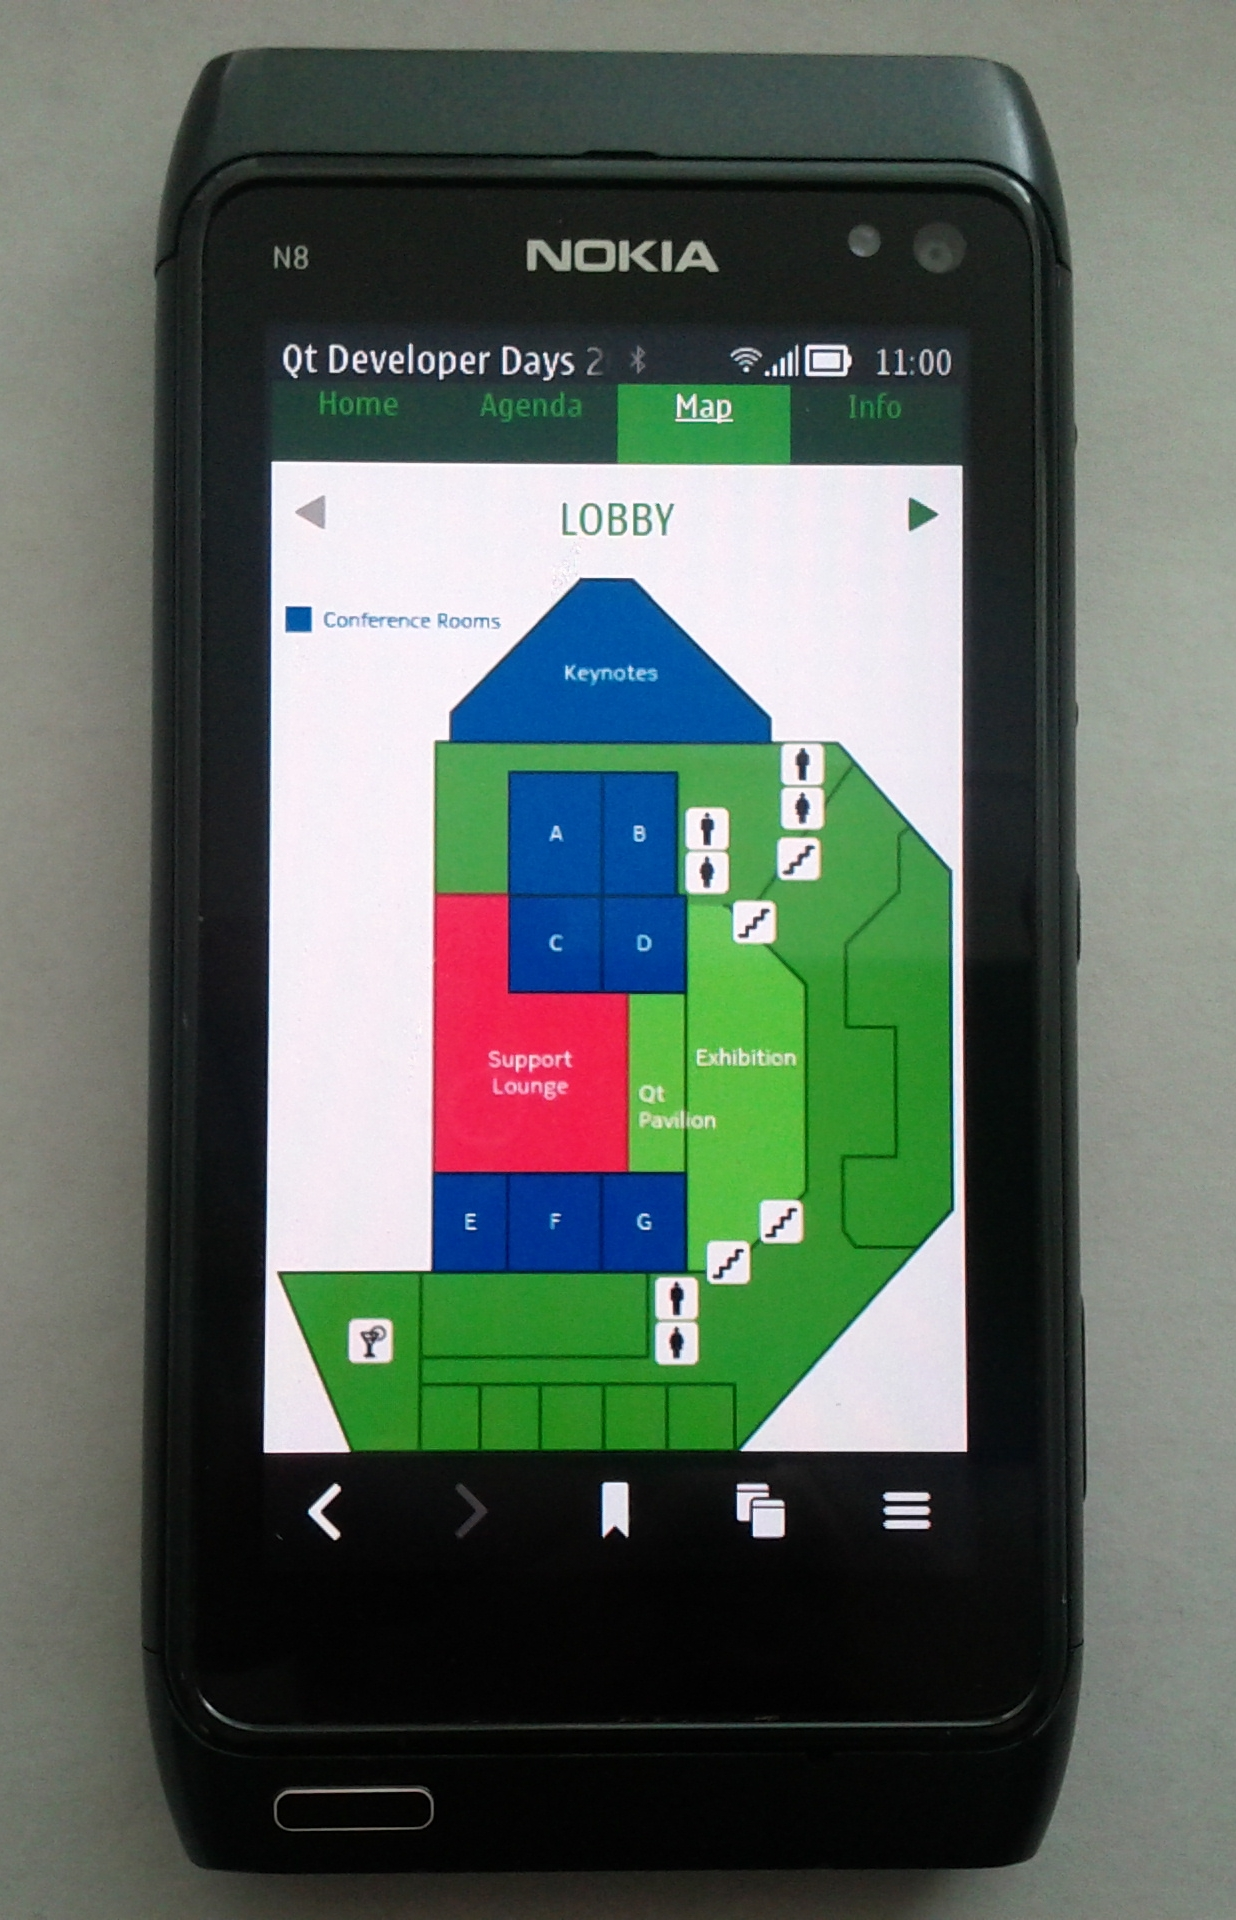
\includegraphics[width=0.5\textwidth]{images/nokia-map.jpg}
    \caption{Floor map view on a device running Nokia Belle
      (previously Symbian Belle).}
    \label{figure:nokia-map.jpg}
  \end{center}
\end{figure}

\section{Handling Different Orientations}

As shown in the previous section, screen sizes and dimensions vary
between devices. In addition to handling different resolutions and
dimensions, we must also handle screen orientation changes. The width
and height of the touch screens are usually different, and the user
can hold the device either in portrait or in landscape mode and at any
point switch between the two (see requirement 2 in
Section~\ref{section:devdays-requirements}).

In the conference application, I wanted to have different header and
footer background images for different orientations. I also needed to
redraw the agenda view when the screen width changes since the items
on the schedule needed to be dynamically positioned to the available
space.

Mobile browsers fire an 'orientationchange' event whenever the device
orientation changes. The application listened to this event, inferred
the orientation from the screen dimensions, and executed the wanted
functionality for the event. I also had to do a fallback for Mobile
\abbr{IE} browser to listen to the window resize event because the
browser does not support the orientation change event.

\section{Handling Mobile Networks}
\label{section:handling-networks}

One of the biggest problems in mobile web applications is the network
that is often slow and unreliable \cite{zandy2002reliable}. Our
conference application was designed for a context where the
application cannot trust on the networking but should still manage to
handle interactions and persist application state (see requirement 4
in Section~\ref{section:devdays-requirements}). Also being a
conference where people come from around the world, the network data
transfer cost might be surprisingly high, and thus bandwidth should be
saved whenever possible.

\subsection{Minimizing Data Transfer}

The best approach to minimize data that needs to be transferred is to
avoid the transfer whenever possible, for example, with proper
caching. However, with initial download or with dynamic data, the
second best option is to minimize the size of the data needed to be
transferred.

First, I made sure the data was minimized and compressed with
Gzip. Second, using \abbr{JSON} instead of \abbr{XML} in \abbr{Ajax}
requests saves bandwidth \cite{charland2011mobile} and needed effort
from the browser to process the data. Third, using the offline
manifest ensured that the application assets and data needed to be
downloaded only once, and using localStorage I could store the
application state locally to the browser avoiding the network
completely.

\subsection{Caching}

Caching on different levels of the application stack is one of the
most important optimizations that should be done. Caching can be done
in the client side using HTML5 storage APIs (see
Section~\ref{section:datastorage}), on the HTTP level letting the
browser handle it complying to the HTTP caching header semantics, or
in various levels of the backend application stack.

In the conference application, I put the most focus on the HTTP
caching. Following the performance guidelines specified in
Section~\ref{section:performance-guidelines}, I created unique
\abbr{URLs} for all different versions of all static resources
(images, CSS files, JavaScript files, and the AppCache manifest file)
and set a far future expires header to them. This way I could tell the
browser to cache all resources as far as possible and updating the
resources was handled by changing the version number in their
corresponding URLs.

In addition to the HTTP-level caching, using the AppCache manifest
file to tell the browser to cache all needed resources to a more
persistent offline cache, which minimized needed downloads on
application startup if the resources were already in the cache (see
requirement 4 in Section~\ref{section:devdays-requirements}). The
effect of this was clearly seen in the application log files, where
the manifest file was first downloaded with the referenced other files
on the first page load, but on subsequent page loads only the manifest
file was requested for changes.

Client side caching was used in saving the user specific state in the
conference application and experimented with the JSONCache library
specified in Section~\ref{section:jsoncache}. Using localStorage, I
could persist data in the browser and avoid networking if the cached
data is still relevant.

JSONCache handles the localStorage caching automatically, with only
user configuration needed for setting the data lifetime. Every time
the data is requested again, the local cache is checked first, and
networking can be avoided altogether (see requirement 7 in
Section~\ref{section:jsoncache-requirements}).

\subsection{Preloading}

One way to prevent user interface slowness due to flaky networks is to
preload resources and data that is expected to be used later on. In
the conference application I predownloaded background images and other
graphics in the application initialization.

For example, downloading the header and footer background images for
both orientations made the device orientation change more responsive
because otherwise the browser would have started to download the
images after the orientation had already changed. With preloaded
images the browser just had to switch the image and render it
instantly without any networking.

\subsection{Offline Support}

Using HTML5 AppCache offline manifest file and storing application
state in localStorage, I provided full offline compatibility for the
conference application. With the offline manifest, I specified the
needed resources for all device types as categorized by the rules
defined in Section~\ref{subsection:device-detection}. The offline
cache also made subsequent application startups faster since the cache
is more persistent than the HTTP cache in browsers.

The offline support was especially critical for the conference
application since the conference ended up having indeed a very bad
wireless network.  Without the offline support, users would not have
been able to check the session schedule during the conference.

However, the only thing needing the network was the session feedback
functionality. The application had a feedback form for all sessions,
and the submitted data was persisted in the backend. In offline mode,
this functionality was not available. Going further, I could extend
the offline support by saving the given feedback, for example, to
localStorage and sending it later to the backend server when the
network connection is open again.

I had some problems in developing the application when using the
offline manifest. In development mode, I want changes to be shown
immediately, and I had to conditionally use the offline manifest based
on the environment.

Using the offline manifest poses several additional problems. First,
the whole cache is made invalid if only a single resource returns a
404 Not Found HTTP status code. Second, if there are updates in the
cache, the updates are indicated in the JavaScript events, but the
updated resources are available only in the second page load after the
updates. Therefore, updates do not show up immediately when the
application is refreshed, and I had to show an additional confirm
dialog for informing the user about updates so that they could refresh
the page again. This has a somewhat noticeable impact on the
application user experience, but was seen as a needed compromise to
get the latest conference schedule data and interface updates.

\subsection{Handling Interruptions}

Small interruptions are common in mobile networks
\cite{zandy2002reliable}. For example, the user might have a stable
network connection, but after walking into an elevator the connection
drops for a moment. Then after exiting the elevator the device
reconnects to the network. Applications should expect these
interruptions and should not fail immediately with brief interruptions
in flaky networks.

JSONCache library introduced in Section~\ref{section:jsoncache} had a
functionality to overcome these issues. The library tries to download
the requested data multiple times, and fails only when the configured
maximum attempt count is reached (see requirement 8 in
Section~\ref{section:jsoncache-requirements}). With every iteration, a
timeout is set for a new request, and the timeout is increased after
each failed attempt. This approach works very well, and together with
localStorage caching lets data updates circumvent small network
interruptions failing only when the network connection seems to be
completely down.

\section{Animations}
\label{section:animations}

Animation and transitions, if not overused, can be a valuable addition
to the user experience of an application. For example, having a simple
sliding animation between different views makes the application more
uniform and pleasing to the eye.

There are several ways to animate elements in a web application. The
simplest is to use \abbr{CSS3} animations (see
Section~\ref{section:css}). However, the performance of the animations
is not yet good enough for a cross-platform mobile application. I
tried to animate the view changes in our conference application, but
even a simple cross-fade did not have good enough performance in all
target platforms.

Using progressive enhancement techniques (see
Section~\ref{subsection:progressive-enhancement}) I could have
provided enhanced experience for the platforms that support animations
well, but only iOS devices performed well enough, so for simplicity I
did not use any animations.

\section{Following JavaScript Best Practices}
\label{section:js-best-practices}

There are lots of best practices and conventions that have been
developed by the web developer community. A lot of these tried and
tested techniques are outlined in the HTML5 Mobile
Boilerplate\footnote{\url{http://html5boilerplate.com/mobile}} that I
used as a base for the conference application. Here I present some
techniques and tools that help to improve application performance and
reduce bugs.

\subsection{JSLint}

JSLint\footnote{\url{http://jslint.com/}} is a code quality tool for
JavaScript. There are several JavaScript features that are suboptimal
for performance or code maintainability
\cite{crockford2008javascript}. JSLint also checks for JavaScript
syntax and convention violations, which is valuable because the code
will be sent in the source form to be interpreted by the browser.

I had automatic JSLint checking integrated in the GNU
Emacs\footnote{\url{http://www.gnu.org/software/emacs/}} editor that I
used for all JavaScript programming, which helped to notice common
errors as early as possible and made the code cleaner.

\subsection{Lazy initialization}

Postponing work as long as possible is a valuable optimization
technique. In lazy initialization, initialization work is minimized in
application startup to render the initial view fast. Additional views
are then initialized only when they are requested.

Implementing lazy initialization needs more work than simply doing all
initialization work in the application startup, but the received
benefits are worth the extra effort. In the conference application I
tried to postpone all work to be done as late as possible and doing as
little work as possible for faster execution.

\subsection{Efficient DOM Manipulation}

After mobile network issues and data transfers, DOM manipulation is
one of the first things to optimize for performance. There are several
known performance issues, but the biggest and most common issue is
updating a number of elements at once. \cite{zakas2010high}

The application might, for example, refresh the contents of a list,
and with an overly simplistic (but still common) implementation would
create the list items and add them to the list container one by
one. This causes the browser to reflow the page after each insertion
and might add up to user interface artifacts and
slowness. \cite{zakas2010high}

One approach to handle updating several elements at once is to use
document fragments. With document fragments, several elements can be
added to one fragment, which can then be added to the element
container. This has no effect on the \abbr{DOM} tree itself, but it
requires only one reflow from the browser. One other solution is
hiding the container while its contents is modified, and showing it
after the modifications are done. \cite{zakas2010high}

I used these techniques in the conference application to minimize user
interface reflows to improve the perceived performance.

\subsection{Efficient Event Handling}

In an interactive web application, there are lots of event listeners
and handler functions. For example, a list of dozens or hundreds of
items might have one or even several event handlers for each item in
the list. This obviously becomes a burden especially in mobile devices
with limited processing power and memory.

One way to minimize event listeners is to use event delegation
\cite{zakas2010high}. In event delegation only one event listener is
attached to a parent element of the elements that we want to
observe. Then, in the parent event handler we check the target element
of the event and execute the wanted functionality based on the target.

One other optimization for touch screens is to use native touch events
instead of traditional mouse events such as click. Mobile browsers
typically have a delay or 300 milliseconds after a touchstart event
until the click event is
fired\footnote{\url{http://code.google.com/mobile/articles/fast_buttons.html}}. This
is because the browser waits if the user is doing a double tap instead
of a single tap and a delay is needed before a double tap can be
excluded. If we bind our event handlers to the touch events instead of
click events, we can immediately dismiss this delay altogether and
make the user interface components a lot more responsive.

I used event delegation and touch events, for example, in the main
navigation of the conference application to get the best performance
and responsiveness in changing the page views. I also used touch
events in the session rating form seen in
Figure~\ref{figure:android-feedback-stars.jpg}.

\begin{figure}[h!]
  \begin{center}
    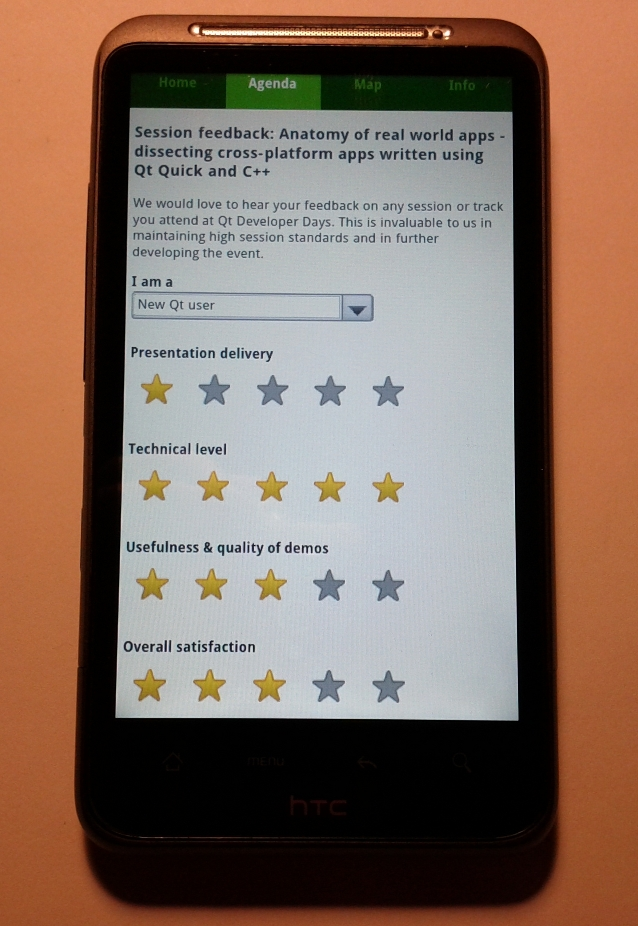
\includegraphics[width=0.6\textwidth]{images/android-feedback-stars.jpg}
    \caption{Touchable session rating stars on a device running Android.}
    \label{figure:android-feedback-stars.jpg}
  \end{center}
\end{figure}

\section{Performance Analysis}
\label{section:performance-analysis}

I made a quantitative analysis of the conference application
performance by using two different tools: YSlow and Page Speed. These
tools analyze the performance practices of a web page and provide
optimization guidelines. Many of the rules used in these tools are
derived from or based on the guidelines defined by Souders
\cite{souders2007high, souders2009even} and specified in
Section~\ref{section:performance-guidelines}.

\subsection{YSlow}

YSlow is a website analyzer originally developed by Steve Souders. It
checks the website against the rules defined in
Section~\ref{section:performance-guidelines}. I analyzed the
conference application performance using YSlow. The results of the
analysis are seen in Figure~\ref{figure:yslow-v2-grade.png} and
Figure~\ref{figure:yslow-v2-statistics.png}.

\begin{figure}[h!]
  \begin{center}
    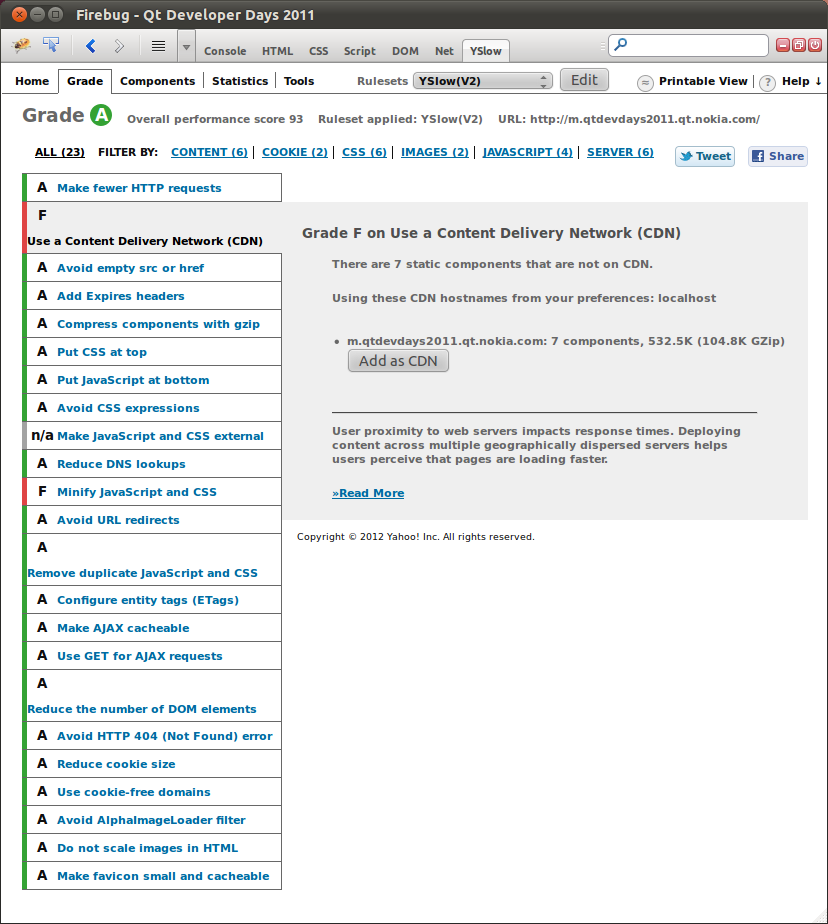
\includegraphics[width=\textwidth]{images/yslow-v2-grade.png}
    \caption{YSlow results grade.}
    \label{figure:yslow-v2-grade.png}
  \end{center}
\end{figure}

\begin{figure}[h!]
  \begin{center}
    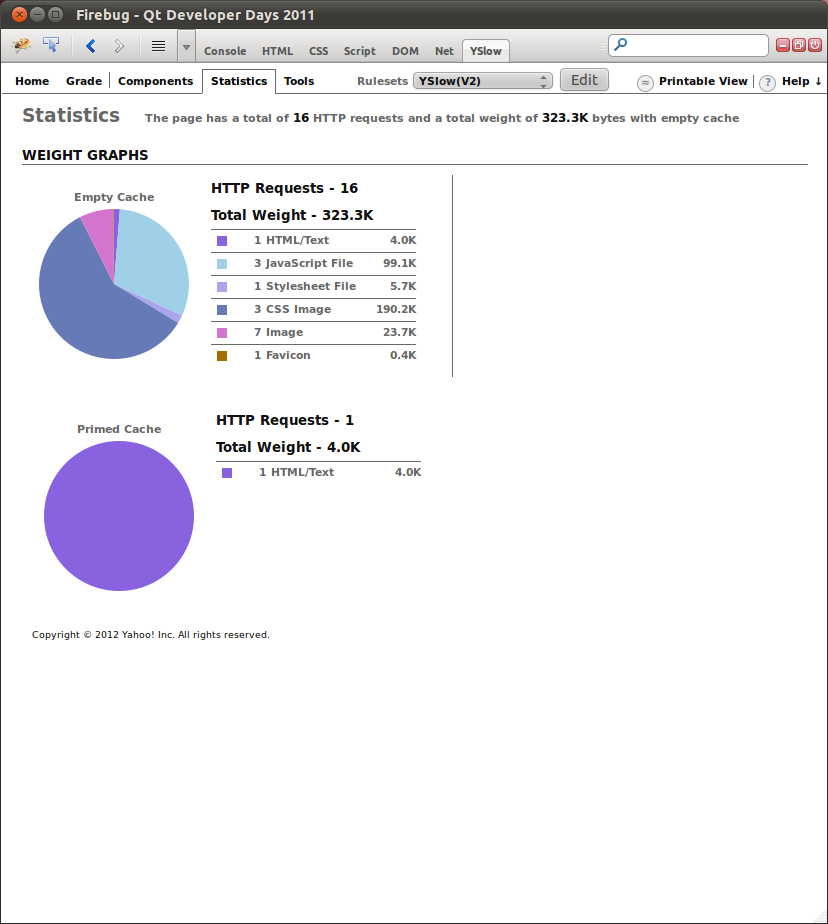
\includegraphics[width=\textwidth]{images/yslow-v2-statistics.png}
    \caption{YSlow results statistics.}
    \label{figure:yslow-v2-statistics.png}
  \end{center}
\end{figure}

The only sections where an A grade (best grade) was not achieved, were
in ``Use a Content Delivery Network'' and in ``Minify JavaScript and
CSS''. The \abbr{CDN} notice was not seen as important because the
application was not designed for world-wide intensive use with lots of
users, but rather for a single conference use with some hundreds of
users.

The minification section notice explained in the details that inline
script tag contents should be minified. This was somewhat a limitation
in the tool itself, since the inline script tags were the HTML
templates for the single-page application JavaScript code. The
\texttt{type} attribute of the tags was
\texttt{text/x-handlebars-template}, which complies with the generic
extension mechanism as specified in the HTML5 specification draft
\cite{HTML5draft}. Thus this was not seen as a problem.

\subsection{Page Speed}

Page Speed\footnote{\url{http://code.google.com/speed/page-speed/}} is
an open-source project by Google for analyzing and optimizing web site
performance best practices. I used the Google Chrome browser extension
to analyze the conference application against the performance rules
defined in Page Speed. The results are shown in
Figure~\ref{figure:devdays-pagespeed.png}.

\begin{figure}[h!]
  \begin{center}
    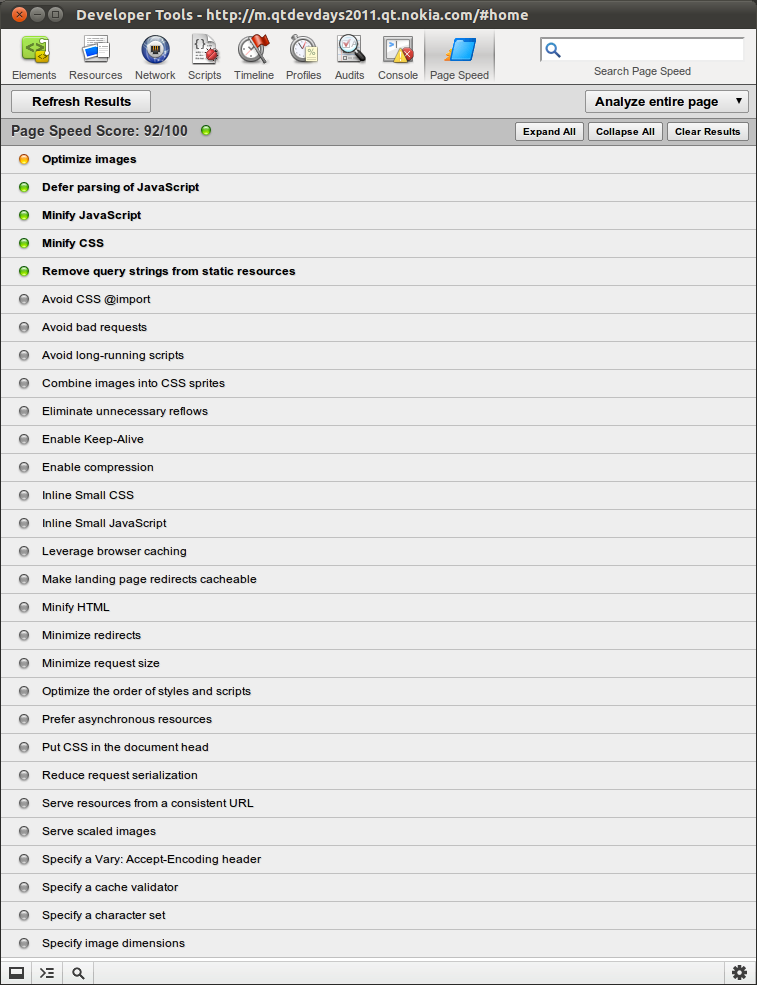
\includegraphics[width=\textwidth]{images/devdays-pagespeed.png}
    \caption{Page Speed results for the conference application.}
    \label{figure:devdays-pagespeed.png}
  \end{center}
\end{figure}

I was very happy with the Page Speed score of 92 out of 100. A lot of
the performance rules analyzed by Page Speed are similar to the
guidelines listed in Section~\ref{section:performance-guidelines}, but
there are also additional rules.

The only real problem in the score was the 'Optimize Images' rule. I
had not optimized the images used in the application, but instead used
the images provided by the designers. Going further, I could have
saved a lot of bandwidth by optimizing the images with tools such as
Pngcrush\footnote{\url{http://pmt.sourceforge.net/pngcrush/}}.

Of the other notes in the results, 'Defer parsing of JavaScript' could
have been avoided by adding a 'defer' attribute to all the script tags
in the document. The reason for this rule is that scripts block page
rendering as defined in
Section~\ref{section:performance-guidelines}. However, since I
followed the guideline 'Put Scripts at the Bottom', this rendering
issue is avoided. The only script in the document head was Modernizr,
which must be included before the page is parsed because it creates
the essential HTML5 tag support for older browsers and must do so
before the tags are parsed.

The 'Minify JavaScript' note was probably due to the Handlebars
templating library not being minified. All the JavaScript libraries
were included in their minified form, but Handlebars library was only
available unminified. I also did not want to minify it myself to avoid
breaking any functionality. All other JavaScript files were minified
and combined to avoid extra HTTP requests.

The 'Minify CSS' note was not seen as important since CSS compression
does not yield big improvements and because the CSS files were already
delivered Gzipped. The 'Remove query strings from static resources'
note means that query parameters like '?123' should be removed from
the end of the \abbr{URLs} because they might not be cached in some
proxies. I did not change this because the query strings in the static
assets were an essential part of our caching strategy.

\section{Summary of Results}

In this chapter, I presented techniques and tools to handle
problematic areas in mobile web development. I used several APIs
defined in HTML5 and related specifications to tackle these practical
challenges.

First challenge was to handle the varying screens and device
form-factors (see requirements 1 and 2 in
Section~\ref{section:devdays-requirements}). Feature detection with
media queries (see Section~\ref{section:css}) and the Modernizr
library proved to be a very practical and working solution for
targeting styles for different device types. Custom \texttt{meta} tags
in the document as well as orientation handling events were invaluable
in setting the viewport dimensions and handling changes in
it. However, screen dimension and orientation handling have lots of
differences between mobile browsers, and due to the differing APIs and
plain browser bugs, handling varying screens and form-factors needed a
lot of testing to get the application layout work properly.

Handling mobile networks is a huge challenge in building mobile web
applications (see requirement 4 in
Section~\ref{section:devdays-requirements}). I presented many
solutions such as minimizing data transfer, caching on different
application layers, preloading resources, and adding offline support
with HTML5 APIs. These techniques need a lot of know-how and
experience, and might not be trivial to implement.

The offline capabilities defined in HTML5 specifications were very
valuable and adding offline support ended up being rather simple for a
single-page application. However, handling interruptions and
unreliable networks is more complex, which is why I developed the
JSONCache utility library for caching and fetching data multiple times
in unreliable networks (see requirements 7 and 8 in
Section~\ref{section:jsoncache-requirements}). In my testing, the
library worked very well, and using this approach can have a big
effect on the end-user experience.

Defining cross-browser stylesheets for different mobile and tablet
devices is hard. The CSS support varies between platforms and platform
versions, and usually the group of target devices for testing ends up
being very large. Animations were a huge pain point in CSS. Adding an
animation is very simple using the CSS3 animation rules, but the
performance in mobile browsers is very poor to say the least. This is
why I dropped all animations from the page changes in the conference
application. I hope this is one area where future platform and mobile
browser updates put focus on, since animations are an essential part
of the user experience of an application.

I provided many techniques for efficient scripting in mobile web
applications. In my view, the architecture as well as the DOM and
event handling are the most important areas for performance
optimization. I provided solutions like lazy initialization, document
fragments, and event delegation as well as introduced the JSLint tool
for automatically checking code quality.

Last, I did a quantitative web performance best practices analysis on
the conference application. Using the YSlow and Page Speed tools, I
got very high scores and explained the areas for further
improvement. These automatic tools are valuable in optimizing the
overall performance, since they point out the most problematic areas
for improvement, and many of the solutions can be very simple, such as
configuring the web server without even touching the application
itself.

To answer the research questions posed in
Section~\ref{section:research-questions}, I sum up as follows:

\begin{itemize}
\item \textbf{RQ1}: \textit{What are the main problem areas in mobile
  web development?}

  The main problems are targeting different types and sizes of screens
  and resolutions, handling the unreliable networks and offline modes,
  and user interface performance, especially with animations.

\item \textbf{RQ2}: \textit{Do HTML5 and related specifications solve
  these problems?}

  The specifications offer a good way to target different screens with
  media queries, but browsers have a lot of differences that have to
  be tested for.

  Offline support is relatively easy to provide, but handling
  interruptions and unreliability have to be tailored in the
  application architecture.

  Performance optimization is the job of the application developer,
  and animation performance is hard to optimize for, leaving future
  updates for the browsers as the only viable option.

\item \textbf{RQ3}: \textit{What other practical means do we have to
  solve these problems?}

  Custom meta tags are very useful for configuring the viewport and
  sound architectural choices and best practices help optimizing the
  application performance.

\end{itemize}
